\documentclass[a4paper, 12pt]{article}
\usepackage[utf8]{inputenc}
\usepackage[T2A]{fontenc}
\usepackage[english,russian]{babel}

\usepackage{authblk}  % для более гибкой работы с авторами
\usepackage{geometry} % если понадобится настроить поля
\usepackage{amssymb} % mathbb etc.
\usepackage{amsmath} % boldsymbol etc.
\usepackage{graphicx} % path to plot
\usepackage{algorithmic}
\usepackage{algorithm}
\usepackage{subcaption} % for subfigures
\usepackage[style=numeric-comp,sorting=none,maxnames=1,giveninits=true,doi=false,url=false,eprint=false]{biblatex} % for nice cites
\usepackage{cleveref}
\usepackage{etoolbox}

\defbibheading{bibliography}{
  \section*{\centering\small References}

  \vspace{-0.8em} % optional: reduces space after the title
}
\renewcommand*{\bibfont}{\small} % smaller than \small (usually 9pt)

\addbibresource{../article/draft_lib.bib}  % with .bib extension

% Title compactness
%\usepackage{titling}
%\setlength{\droptitle}{-2em}

% Custom bibliography style
\DeclareFieldFormat{title}{#1}
\DeclareFieldFormat{journaltitle}{#1}
\DeclareFieldFormat{volume}{\textbf{#1}}
\DeclareFieldFormat{number}{(#1)}
\DeclareFieldFormat{pages}{#1}

\renewbibmacro*{journal+issuetitle}{%
  \usebibmacro{journal}%
  \setunit*{\addcomma\space}%
  \iffieldundef{volume}{}{
    \printfield{volume}%
    \setunit{\addcolon\space}%
    \printfield{number}%
    \setunit{\addcolon\space}%
    \printfield{pages}}%
  \newunit}

\renewbibmacro*{volume+number+eid}{%
  \printfield{volume}%
  \setunit{\addcolon\space}%
  \printfield{number}%
  \setunit{\addcolon\space}%
  \printfield{pages}}

% Compact bibliography spacing
\setlength\bibitemsep{0pt plus 0.3ex}
\setlength\biblabelsep{0.5em}
\setlength{\bibnamesep}{0pt}
\setlength{\bibinitsep}{0pt}

\geometry{margin=2.5cm} % стандартные поля


% remove and for authors
\renewcommand\Authfont{\small} % размер шрифта для авторов
\renewcommand\Affilfont{\small} % размер шрифта для аффилиаций
\renewcommand\Authsep{, } % разделитель между авторами
\renewcommand\Authand{, } % разделитель между последним и предпоследним автором

% Reduce title spacing
\makeatletter
\renewcommand\maketitle{\par
  \begingroup
    \renewcommand\thefootnote{\@fnsymbol\c@footnote}%
    \def\@makefnmark{\rlap{\@textsuperscript{\normalfont\@thefnmark}}}%
    \long\def\@makefntext##1{\parindent 1em\noindent
            \hb@xt@1.8em{%
                \hss\@textsuperscript{\normalfont\@thefnmark}}##1}%
    \if@twocolumn
      \ifnum \col@number=\@ne
        \@maketitle
      \else
        \twocolumn[\@maketitle]%
      \fi
    \else
      \newpage
      \global\@topnum\z@
      \@maketitle
    \fi
    \thispagestyle{empty}\@thanks
  \endgroup
  \setcounter{footnote}{0}%
  \global\let\thanks\relax
  \global\let\maketitle\relax
  \global\let\@maketitle\relax
  \global\let\@thanks\@empty
  \global\let\@author\@empty
  \global\let\@date\@empty
  \global\let\@title\@empty
  \global\let\title\relax
  \global\let\author\relax
  \global\let\date\relax
  \global\let\and\relax
}
\makeatother

\makeatletter % small title and authors
\renewcommand{\maketitle}{
  \begin{center}
    \fontsize{15}{12}\selectfont
    \textbf{\@title} \\
    \vspace{0.5em}
    \@author \\
    \vspace{0.5em}
    \@date
  \end{center}
  \vspace{-0.5em}
}
\makeatother

% Title and author info (must be before \begin{document})
\title{\textbf{Differentially private modification of SignSGD}}
\author[]{A.Yu.~Kravatskiy}
\author[]{A.A.~Pliusnin}
\author[]{S.A.~Chezhegov}
\author[]{A.N.~Beznosikov}
\affil[]{Moscow Institute of Physics and Technology}
\date{} % убираем дату

\newcommand{\eps}{\varepsilon}
\newcommand{\renyi}{R\'enyi}

\graphicspath{ {fig/} {../figs/} }

\begin{document}

\selectlanguage{english}
\noindent\foreignlanguage{russian}{УДК ?}\vspace{-2em}
\maketitle
Large models requiring more and more data for training, federating learning has become indispensable like never before. To use potentially sensitive user data for training the model, one has to guarantee its privacy. The gold standard for data privacy is $(\eps, \delta)$-differential privacy \cite{Dwork2014} of \emph{mechanism}, which guarantees that that probabilities $p_1$ and $p_2$ of any response of the mechanism on datasets $D_1$ and $D_2$ respectively that differ only in one entry satisfy the relations $\frac{p_1}{p_2} \leq e^{\eps} + \delta$ and $\frac{p_2}{p_1} \leq e^{\eps} + \delta$. In the case of federated learning, the mechanism is all the outputs from the user's side, i.e. all the gradient data that they send to the server. For neural networks, recommended $\eps = 1$, $\delta = 10^{-5}$. 

Another constraint of federated learning is a high communication cost. To reduce it, one may send not the whole gradient, but only signs of each coordinate, thus reducing the cost in $32/2 = 16$ times. The standard algorithm that utilizes this technique is Sign-SGD \cite{Bernstein2018}. This algorithm with \emph{majority voting} (amidst workers that participate in the learning process) is not only communication-efficient, but also has proved to be resistant to heavy-tailed noise and converge with high probability \cite{Kornilov2025}.

Initially, we planned to provide theoretical guarantees of convergence, as in \cite{Kornilov2025}, for DPSignSGD, a differentially private modification of SignSGD \cite{Jin2020}. However, on closer inspection, it turned out that that the algorithm is not truly differentially private. The authors have shown $(\eps, \delta)$-privacy of a single use of DPSignSGD, which means only $(T\eps, T\delta)$-privacy for the whole procedure ($T$ iterations). Moreover, they did not prove the convergence of DPSignSGD.

Thus, we had to construct our own DPSignSGD. We use the same Gaussian noise mechanism, adding $\mathcal{N}(0,\sigma^2\mathbb{I}^d)$ noise, to ensure differential privacy. However, to make the most out of composition of mechanisms (the single mechanism being a sign of the gradient sent) and to enhance privacy, we add Bernoulli subsampling mechanism (one samples each of the elements with probability $q$) with proved $(\alpha, \eps_R)$-\renyi\ differential privacy \cite{mironov2019SGM}, which is easily converted to $(\eps, \delta)$-privacy. We use the tighest proved bound for $\eps_R$, which can be computed only numerically:
\begin{equation}\label{eq:renyi_eps_guarantee}
\eps_R = \frac{1}{\alpha - 1} \log\left(\sum_{k=0}^{\alpha} {\alpha \choose k}  (1-q)^{\alpha-k}q^{k} \exp\left(\frac{k^2 - k}{2\sigma^2}\right)\right)
\end{equation}

To preserve privacy, earlier defined $\eps_R$ and $\sigma$ must satisfy:
\begin{equation}\label{eq:renyi_eps_requirement}
\eps_R \leq \eps/T - \frac{\log 1/\delta}{T(\alpha - 1)}
\end{equation}

To find the lowest $\sigma$, we perform grid search, like \cref{fig:grid_sigma}.
\begin{figure}[h]
    \centering
    \begin{subfigure}[b]{0.39\textwidth}
        \centering
        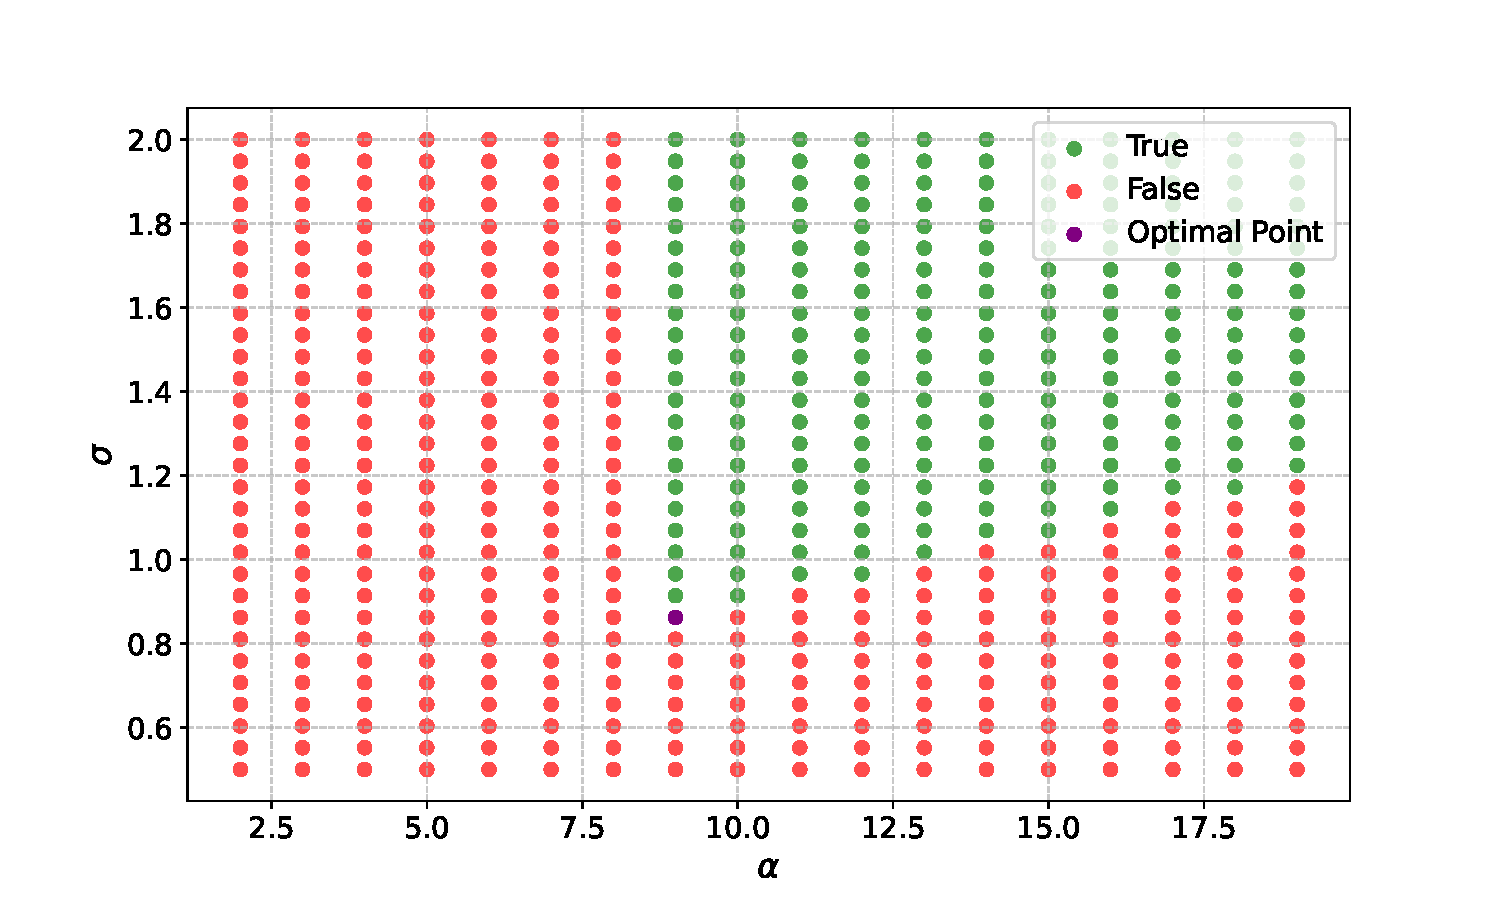
\includegraphics[width=\textwidth]{grid_sigma_to_pres.pdf}
        \caption{Finding the minimal $\sigma$, sampling rate $q = 1/300$, and $T = 1000$}
        \label{fig:grid_sigma}
    \end{subfigure}
    \hfill
    \begin{subfigure}[b]{0.6\textwidth}
        \centering
        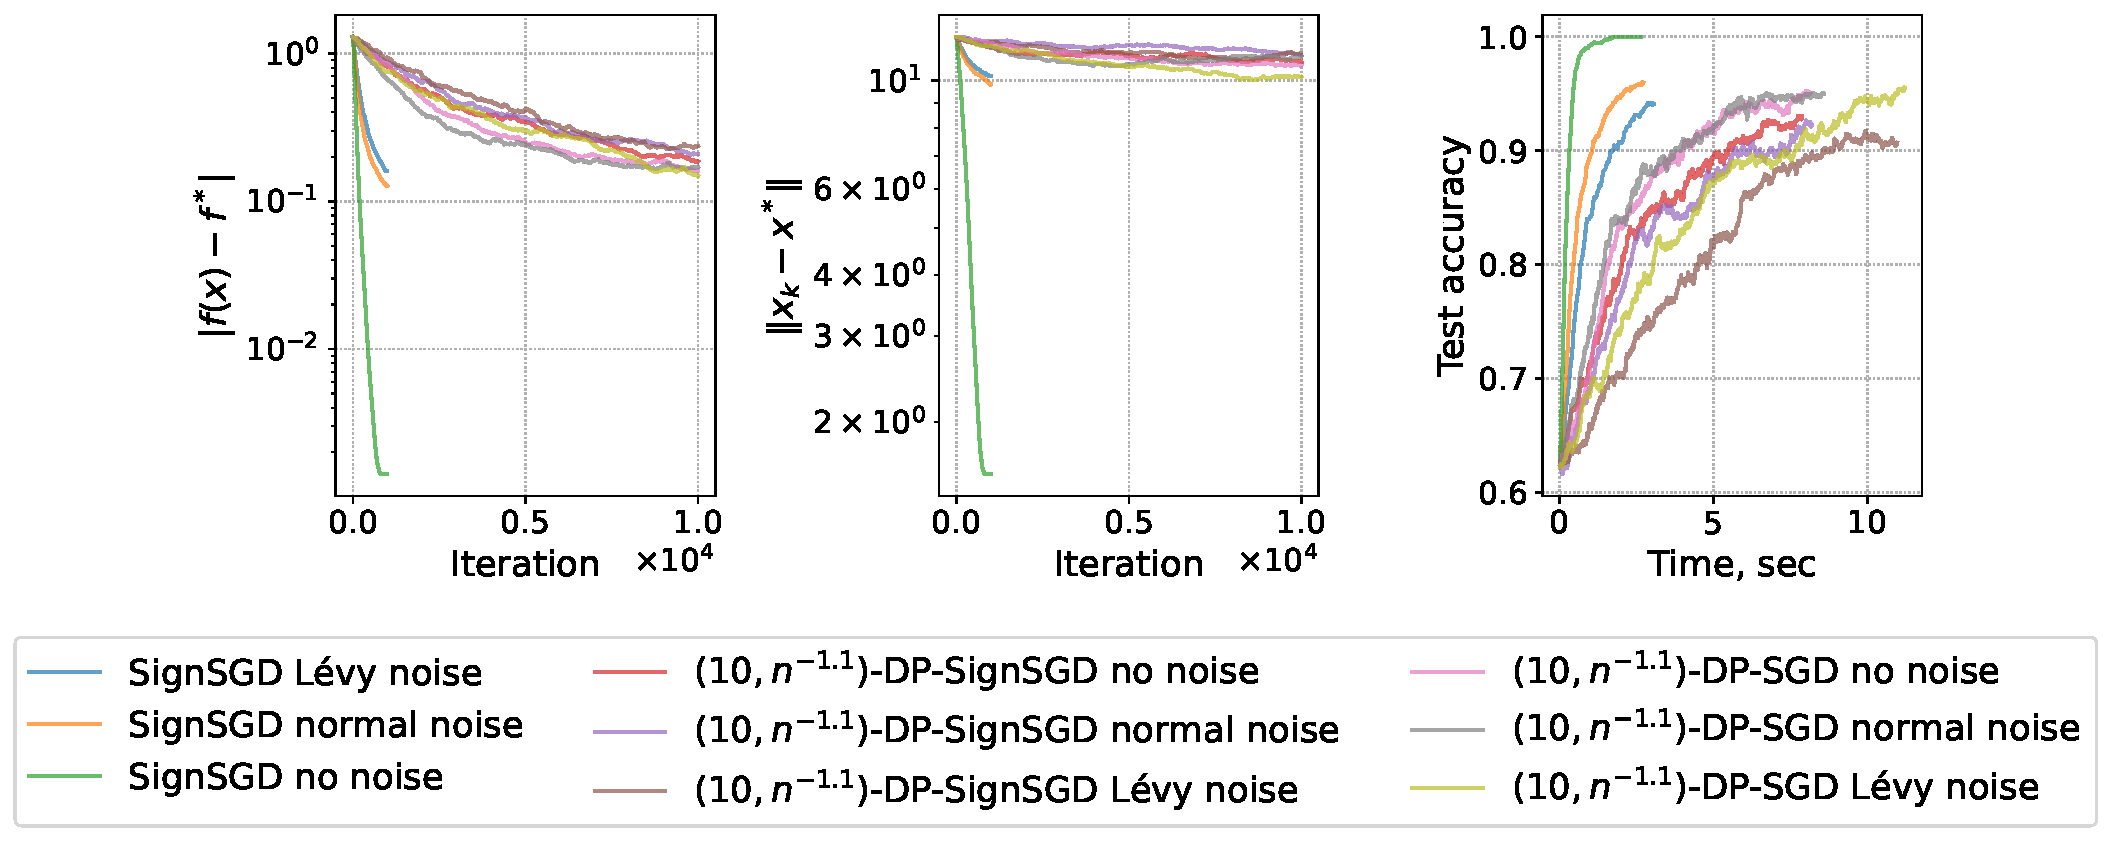
\includegraphics[width=\textwidth]{v28_constant_step/short/v28_constant_step_short.pdf}
        \caption{Logistic regression on UCI Mushroom Dataset with SGD, SignSGD, {\scriptsize DP-SIGN}SGD and different type of noises}
        \label{fig:logreg}
    \end{subfigure}
    \caption{Experimental results}
\end{figure}

Thus, we derive a new DP-SIGN compressor (\cref{dp-sign-precise}), which defines truly private DP-SignSGD. We test it on a regularized logistic regression problem for binary classification \cref{fig:logreg}.


\newcommand{\gradg}{\boldsymbol{g}}
\begin{algorithm}
    \caption{DP-SIGN compressor}
    \label{dp-sign-precise}
    \begin{algorithmic}
        \STATE \textbf{Input}: coordinate $w$, loss function $l$, user database $D$, $(\eps, \delta)$-privacy requirement, number of iterations $T$, sampling rate $q$, clipping level $C$.
        \STATE Prepare subsample $S$: add each element $(x, y) \in D$ with probability $q$.
        \STATE Compute the gradient $\gradg$ of the subsample: $\frac{1}{|S|}\sum_{(x,y)\in S}l(w;(x,y))$. If $S$ is empty, let $\gradg = 0$.
        % \STATE If $||\gradg||_2 > C$: $\gradg = C\frac{\gradg}{||\gradg||_2}$.
        \STATE Grid search $\sigma(q, T, \eps, \delta)$ to satisfy \eqref{eq:renyi_eps_guarantee} and \eqref{eq:renyi_eps_requirement}.
        \STATE $sign_{noised} = sign(\gradg + \mathcal{N}(0,\sigma)^2\mathbb{I}^d)$
        % \STATE $\gradg_{priv}$ = $\gradg + \mathcal{N}(0,(C\sigma)^2\mathbb{I}^d)$
        \STATE \textbf{Output}: $sign(sign_{noised})$
    \end{algorithmic}
\end{algorithm}

Also we test it on MLP and CNN for hand-written digit classification from MNIST dataset. On a single worker, we reach 70\% accuracy when we run the algorithm for 30 000 iterations, and 40\% in 2 000 iterations. The main obstacle to reaching high accuracy is a Gaussian noise, inherent in private algorithms. Even with a skillful privacy accounting, it causes a tradeoff: precision vs max iteration number that still preserves privacy.

That being said, DP-SignSGD promises to be far more private than we calculate. Indeed, the sign mechanism returns not all values in range [-1, 1], but only 1 and -1, which naturally should add more privacy guarantees. Moreover, even the gradients might be private to some extent in respect to the user dataset. Estimating the impact of these features of the mechanism might produce far more feasible algorithms.

Interestingly, DP-SignSGD can be easily adapted to any new tighter privacy guarante: lowering $\sigma$ or raising $T$ directly improves training results. At present, the pressing need concerning DP-SignSGD with $\sigma$ noise and sampling probability $q$ is to establish theoretical guarantees of its convergence. To the best of our knowledge, none of the existing works contain theoretical analysis of application of subsampling mechanism to optimization algorithms.

\vspace{-2em}
\printbibliography[heading=bibliography]


\end{document}
